% Metódy inžinierskej práce

\documentclass[10pt,slovak,a4paper]{article}

\usepackage[slovak]{babel}
%\usepackage[T1]{fontenc}
\usepackage[IL2]{fontenc} % lepšia sadzba písmena Ľ než v T1
\usepackage[utf8]{inputenc}
\usepackage{graphicx}
\usepackage{url} % príkaz \url na formátovanie URL
\usepackage{hyperref} % odkazy v texte budú aktívne (pri niektorých triedach dokumentov spôsobuje posun textu)

\usepackage{cite}
%\usepackage{times}

\pagestyle{plain}

\title{Sekvenčné UML Diagramy\thanks{Semestrálny projekt v predmete Metódy inžinierskej práce, ak. rok 2021/22, vedenie: Ing. Ján Lúčanský}}

\author{Kristián Lukacsovics\\[2pt]
    {\small Slovenská technická univerzita v Bratislave}\\
    {\small Fakulta informatiky a informačných technológií}\\
    {\small \texttt{xlukacsovics@stuba.sk}}
    }

\date{\small 5.11.2021} % upravte

\providecommand{\abstr}[1]{\textbf{\textit{Abstrakt---}} #1}
\providecommand{\keywords}[1]{\textbf{\textit{Klúčové slová---}} #1}

\begin{document}

\maketitle

\abstr{Tento článok sa zameriava na opis sekvenčných UML diagramov\ldots\newline}
\indent\keywords{Unified Modeling Language, Sekvenčný diagram, Objekt, Správa}

\section{Úvod}
UML, celým názvom Unified Modeling Language, je objektovo-orientovaný modelovací jazyk pre softvérové programy. \cite{eriksson98}
Existuje niekoľko typov UML diagramov, sekvenčné diagramy sú jedným z nich. Všetky tieto diagramy slúžia na
abstraktný opis správania sa jednotlivých častí počítačového programu. Každý jeden typ sa sústreďuje na opis
rôznych vlastností kódu. Cieľom sekvenčných diagramov je opis interakcie medzi objektami programu, s tým, že sa
berie ohľad na poradie vykonávaného postupu. \cite{petraq14}

\section{Komunikácia objektov} \label{nejaka}

\noindent Objekty si navzájom posielajú správy (požiadavky) medzi sebou. Tieto
správy medzi objektami sa v diagrame zaznačia ako horizontálne šípky. Smer týchto šípok určuje odosielateľa a
príjemcu (na strane, kde je šípka, je príjemca). Samotné objekty sa značia ako vertikálne čiary, s tým, že
na vrchu tejto čiary je meno objektu. Tieto vertikálne čiary značia aj dĺžku života objektov. Úseky, kde sú
čiary prerušované, značia časové úseky programu, kde dané objekty ešte neboli vytvorené, resp. už boli odstránené. \newline

\noindent Objekty si môžu poslať správy aj pre seba. Takéto správy sa nazývajú reflexívne správy. 
Ako už bolo spomenuté, poradie týchto správ je dôležité. Zmena poradia môže zmeniť korektnosť programu
v niektorých prípadoch. \cite{petraq14}  \newline

\begin{figure*}[tbh]
\centering
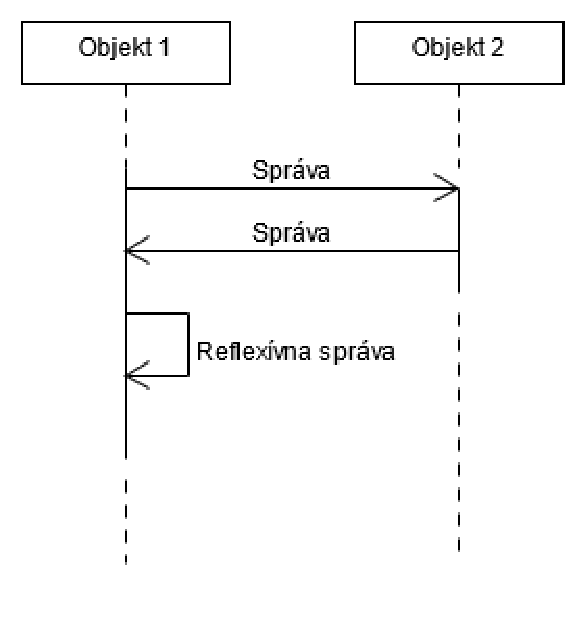
\includegraphics[scale=0.7]{seq_diagram.pdf}
\caption{Ukážka sekvenčného diagramu.}
\end{figure*}

\noindent Na obr. 1 môžeme vidieť veľmi jednoduchú ukážku sekvenčného UML diagramu.

\section{Využitie}
Cieľom UML diagramov, vo všeobecnosti, je poskytnúť ucelenejšie a jednoduchšie zobrazenie fungovania softvéru, tak, aby tomu porozumeli aj laici. 
Problém je v tom, že sa väčšinou softvér dizajnuje najprv ako UML diagram, a až potom sa píše samotný kód programu. Keďže UML diagramy používajú objektovo-orientovaný princíp, tak aj kód programu musí byť písaný objektovo-orientovane. \cite{eriksson98}
Ja, osobne, nie som veľký zastánca objektovo-orientovaného programovania. Objektovo-orientované programovanie ma skôr spomaluje, preto radšej programujem procedurálne. Kvôli tomu, že UML diagramy sú úzko späté so štýlom programovania, som nútený programovať v paradigme, ktorá 
ma robí menej efektívnym. Preto je, podľa mňa, lepšie nemodelovať kód programu podľa nadizajnovaného diagramu, ale robiť to opačne. Fungovanie programu by nemalo mať vplyv na to, akým spôsobom ten kód bol napísaný. Objekty v diagrame nemusia reprezentovať explicitne objekty v kóde, môžu reprezentovať 
iné abstraktné podsystémy programu. Tento spôsob zaručuje aj to, že diagramy môžu byť menej abstraktné, nemusia sa riadiť princípom objektového orientovania. Menej abstraktné diagramy môžu byť užitočné pre programátorov, ktorí pracujú na nižšej úrovni, bližšie k hardvéru. \newline 

\noindent Sekvenčné diagramy sa na tento viacej flexibilnejší postup tvorenia diagramov hodia najviac, podľa mňa. Keďže zachytávajú životnosť objektov a poradie operácií, mnoho operácií sa dá zapísať paralelne. Paralelný zápis môže byť užitočný pre programátorov, keďže aj počítač funguje paralelne. 
Program sa tým pádom môže modelovať podľa toho, ako počítač vykonáva operácie, napr. pomocou vlákien procesora alebo pomocou SIMD registrov procesora. Takýto model môže byť užitočný pre programátorov, ktorí sa sústreďujú na optimalizovanie kódu. 
Takisto sa programy môžu modelovať viac abstraktne ako doteraz, akurát s tým, že výsledné diagramy korektne opíšu fungovanie programu bez toho, aby mali vplyv na štýl písania kódu. \newline

\section{Ďalšia časť}

\begin{figure*}[tbh]
\centering
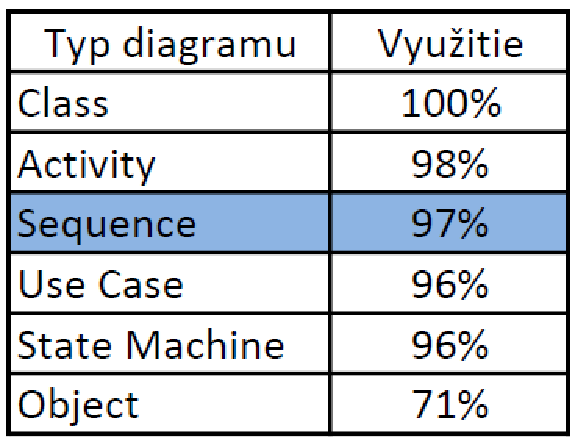
\includegraphics[scale=0.7]{tab.pdf}
\caption{Úroveň využitia jednotlivých typov UML diagramov. \cite{reggio13}}
\end{figure*}

\section{Záver}
\ldots

%\acknowledgement{Ak niekomu chcete poďakovať\ldots}


% týmto sa generuje zoznam literatúry z obsahu súboru literature.bib podľa toho, na čo sa v článku odkazujete
\bibliography{literature}
\bibliographystyle{plain} % prípadne alpha, abbrv alebo hociktorý iný
\end{document}
